\documentclass[12pt, a4paper, titlepage]{report}
\usepackage[a4paper,top=2.5cm,bottom=2cm,left=2cm,right=2cm]{geometry}
\usepackage[italian]{babel}
\usepackage[hidelinks]{hyperref}
\usepackage{graphicx}
\usepackage{algorithm}
\usepackage{capt-of}
\usepackage{amsmath}
\usepackage{longtable}
\usepackage{caption}
\usepackage{booktabs}
\usepackage{algpseudocode}
\usepackage{makecell}
\usepackage[utf8]{inputenc}
\usepackage{fixltx2e}
\usepackage{listings}
\usepackage{hyperref}
\usepackage{makecell}
\usepackage{changepage}
\usepackage{paracol}
\usepackage{siunitx}
\usepackage{lipsum}
\usepackage{float}
\usepackage{subfig}

\usepackage[swapnames]{frontespizio}

\usepackage{fancyhdr}
\usepackage{lastpage}
%\pagestyle{fancy}
%\fancyhf{}
%\cfoot{Pagina \thepage\ di \pageref{LastPage}}

\setcounter{tocdepth}{6}
\setcounter{secnumdepth}{6}
\newcommand\tab[1][1cm]{\hspace*{#1}}
\renewcommand{\thesection}{\arabic{section}}%
\newcommand{\myparagraph}[1]{\paragraph{#1}\mbox{} \mbox{}}
\newcommand{\tommaso}{Tommaso Carraro}
\newcommand{\alberto}{Alberto Bezzon}
	
\begin{document}
	
	\begin{frontespizio}
		\begin{Preambolo*}
			\usepackage{fourier}
		\end{Preambolo*}
		\Universita{Padova}
		\Logo{logo-unipd.png}
		\Dipartimento{Matematica}
		\Scuola{Corso di Mobile Programming and Multimedia}
		\Filigrana [height=7.5cm,before=0.58,after=1.5]{img/delivery-package.png}
		\Titolo{\vspace{8cm}\Huge{Relazione del progetto SmartOrder}}
		\Relatore{Alberto Bezzon 1211016\\Tommaso Carraro 1210937}
		\NRelatore{Studenti}{}
		\Annoaccademico{2018-2019}
	\end{frontespizio}
	
	%\maketitle
	%\pagestyle{empty}
	\setcounter{page}{2}
	\tableofcontents
	\newpage
	\listoffigures
%	\newpage
%	\listoftables
%	\setcounter{table}{0}
	\newpage	    
	\renewcommand*{\arraystretch}{2}
	\pagestyle{fancy}
	\fancyhf{}
	\rhead{Relazione del progetto SmartOrder}
	\lhead{Corso di Mobile Programming and Multimedia \\ Università di Padova}
	\cfoot{\thepage}
	%\setlength{\headsep}{2cm}
	
	\section{Introduzione}
	
	Il progetto consiste nello sviluppo di un'applicazione \textit{mobile}, chiamata \textit{SmartOrder}, progettata per permettere agli utenti registrati di effettuare ordini presso il proprio fornitore. L'applicazione è stata sviluppata esclusivamente per \textit{smartphone}, al momento soltanto per l'ambiente \textit{Android}, utilizzando il \textit{framework cross-platform PhoneGap}. Per l'ambiente \textit{iOS} non è stato possibile realizzare l'applicazione, non essendo il gruppo in possesso di un \textit{Mac}. L'applicazione non prevede una registrazione esplicita, infatti le aziende che intendono acquistare il servizio devono comunicarlo al \textit{team} di \textit{SmartOrder}. Al momento della richiesta devono essere fornite le anagrafiche degli utenti che il fornitore intende registrare e, in questo modo verranno creati gli \textit{account} per tutti gli utenti, compresi di credenziali. Inoltre, devono essere forniti i dati relativi a tutti gli articoli che il fornitore desidera rendere disponibili per gli utenti. Una volta ricevute le credenziali via \textit{e-mail}, gli utenti possono iniziare ad usufruire del servizio. Il tutto sarà perfettamente configurato per fare in modo che ogni utente possa visionare solamente gli articoli venduti dal proprio fornitore. Tramite l'applicazione sarà possibile:
	\begin{itemize}
		\item ricercare prodotti e aggiungerli al carrello;
		\item scansionare il codice a barre di un prodotto che si ha già acquistato per aggiungerlo al carrello più velocemente;
		\item modificare o eliminare i prodotti nel carrello;
		\item inviare un ordine presso il proprio fornitore;
		\item visualizzare le informazioni relative a tutti gli ordini effettuati presso il proprio fornitore.
	\end{itemize}
	L'idea è nata per cercare di soddisfare un bisogno reale. È stato richiesto se fosse possibile velocizzare il processo di rifornimento di libri di una libreria una volta terminati. L'idea è fornire la possibilità di ordinare un libro scansionandone il codice a barre quando esso sta per terminare. La possibilità di aggiungere gli articoli dall'inventario è stata implementata per permettere all'applicazione di essere robusta rispetto all'aggiunta di nuovi clienti, in quanto essi non avendo ancora acquistato prodotti, non hanno la possibilità di scansionare il codice a barre per ordinarli.
	\medskip
	
	\noindent L'applicazione realizzata non presenta la gestione dei pagamenti, in quanto si assume che l'utente abbia un contratto con il proprio fornitore, quindi il denaro viene estratto dal conto corrente al momento dell'ordine.
	
	\section{La scelta del framework}
	
	Per lo sviluppo del progetto si è scelto il \textit{framework cross-platform PhoneGap}, in quanto un membro del gruppo aveva già familiarità con le tecnologie offerte dallo stesso e il suo utilizzo non avrebbe richiesto l'apprendimento di nuove tecnologie. Altri \textit{framework} presi in considerazione, come \textit{Xamarin} e \textit{React Native}, avrebbero richiesto l'apprendimento di \textit{C\#} e \textit{JSX}, rispettivamente, linguaggi poco conosciuti da entrambi i membri del gruppo e il quale apprendimento non avrebbe permesso di concentrarsi maggiormente sulle funzionalità offerte dall'applicazione. Il \textit{framework} scelto ha permesso di:
	\begin{itemize}
		\item implementare l'interfaccia grafica dell'applicazione una sola volta;
		\item accedere ad alcune funzionalità native del dispositivo.
	\end{itemize}
	
	\section{Scelta delle tecnologie web}
	
	Siccome è stato scelto il \textit{framework PhoneGap}, il gruppo ha utilizzato i linguaggi \textit{HTML5}, \textit{CSS3} e \textit{JavaScript}. In particolare, \textit{HTML5} è stato scelto perché include un insieme di funzionalità che permettono di valorizzare le interfacce \textit{mobile}. Alcune di queste evidenziano come \textit{HTML5} sia già per sua natura orientato al \textit{mobile}. In particolare, \textit{HTML5} fornisce \textit{API} per la gestione degli eventi \textit{touch}. Mentre i meccanismi di \textit{input} nei PC consistono per lo più nella tastiera e nel \textit{mouse}, nei dispositivi mobili quasi tutto passa per il \textit{touch screen}, e avere funzionalità comode per gestire questo strumento consente un'interazione più ricca e senza limitazioni per l'utente. Le gestualità da attuare su un \textit{display}, nel mondo \textit{mobile}, costituiscono un vero e proprio linguaggio fondamentale nella \textit{user experience}.
	\medskip
	
	\noindent Ciò che ha favorito la scelta di \textit{CSS3} sono state le \textit{media queries}. Esse permettono di definire regole stilistiche in base alla tipologia del mezzo di visualizzazione, delle sue dimensioni e della sua attuale disposizione (\textit{portrait} o \textit{landscape}). Ciò influisce non solo sull'aspetto esteriore degli elementi ma anche sul loro posizionamento e quindi sulla struttura stessa dell'interfaccia.
	\medskip
	
	\noindent Per quanto riguarda il linguaggio \textit{JavaScript} si è utilizzato \textit{JavaScript} puro, senza l'utilizzo di \textit{framework} o \textit{JQuery}. Una particolarità del linguaggio, detta \textit{AJAX}, ha reso possibile eseguire chiamate all'\textit{API} del servizio \textit{web} di \textit{SmartOrder}. \textit{AJAX}, acronimo di \textit{\textit{Asynchronous JavaScript and XML}}, è una tecnica di sviluppo \textit{software} per la realizzazione di applicazioni \textit{web} interattive (\textit{Rich Internet Application}). Lo sviluppo di applicazioni \textit{HTML} con \textit{AJAX} si basa su uno scambio di dati in \textit{background} fra \textit{web browser} e \textit{server}, che consente l'aggiornamento dinamico di una pagina \textit{web} senza esplicito ricaricamento da parte dell'utente.
		
	\section{Informazioni utili all'utilizzo dell'applicazione}
	
	Per poter utilizzare l'applicazione è necessario essere connessi ad \textit{Internet}, in quanto essa scarica dati da un \textit{server}. Si fa presente che la connessione viene bloccata dalla rete \textit{Eduroam} e \textit{Studenti.math.unipd.it} dell'Università, quindi si consiglia di utilizzare altre reti. Nel caso in cui l'applicazione venisse aperta in assenza di connessione, verrà visualizzato un messaggio d'errore ed essa verrà successivamente chiusa. Per ricevere le \textit{e-mail} al momento dell'invio dell'ordine, è necessario che il proprio indirizzo \textit{e-mail} sia certificato Amazon\footnote{certificazione Amazon: i \textit{server SMTP} di Amazon permettono la spedizione gratuita di \textit{e-mail} ai soli indirizzi certificati. Per poter inviare \textit{e-mail} a tutti gli indirizzi è necessario effettuare l'\textit{upgrade} dell'\textit{account}}. Poiché non sarà possibile quindi ricevere l'\textit{e-mail}, viene di seguito fornito uno \textit{screenshot} della stessa. L'\textit{e-mail} presenta due versioni, a seconda che debba essere inviata all'azienda o all'utente che ha effettuato l'ordine, e contiene un riepilogo dell'ordine effettuato.
	
	\begin{figure}[H] 
		\centering
		\subfloat[\textit{Mail} ricevuta dall'utente]{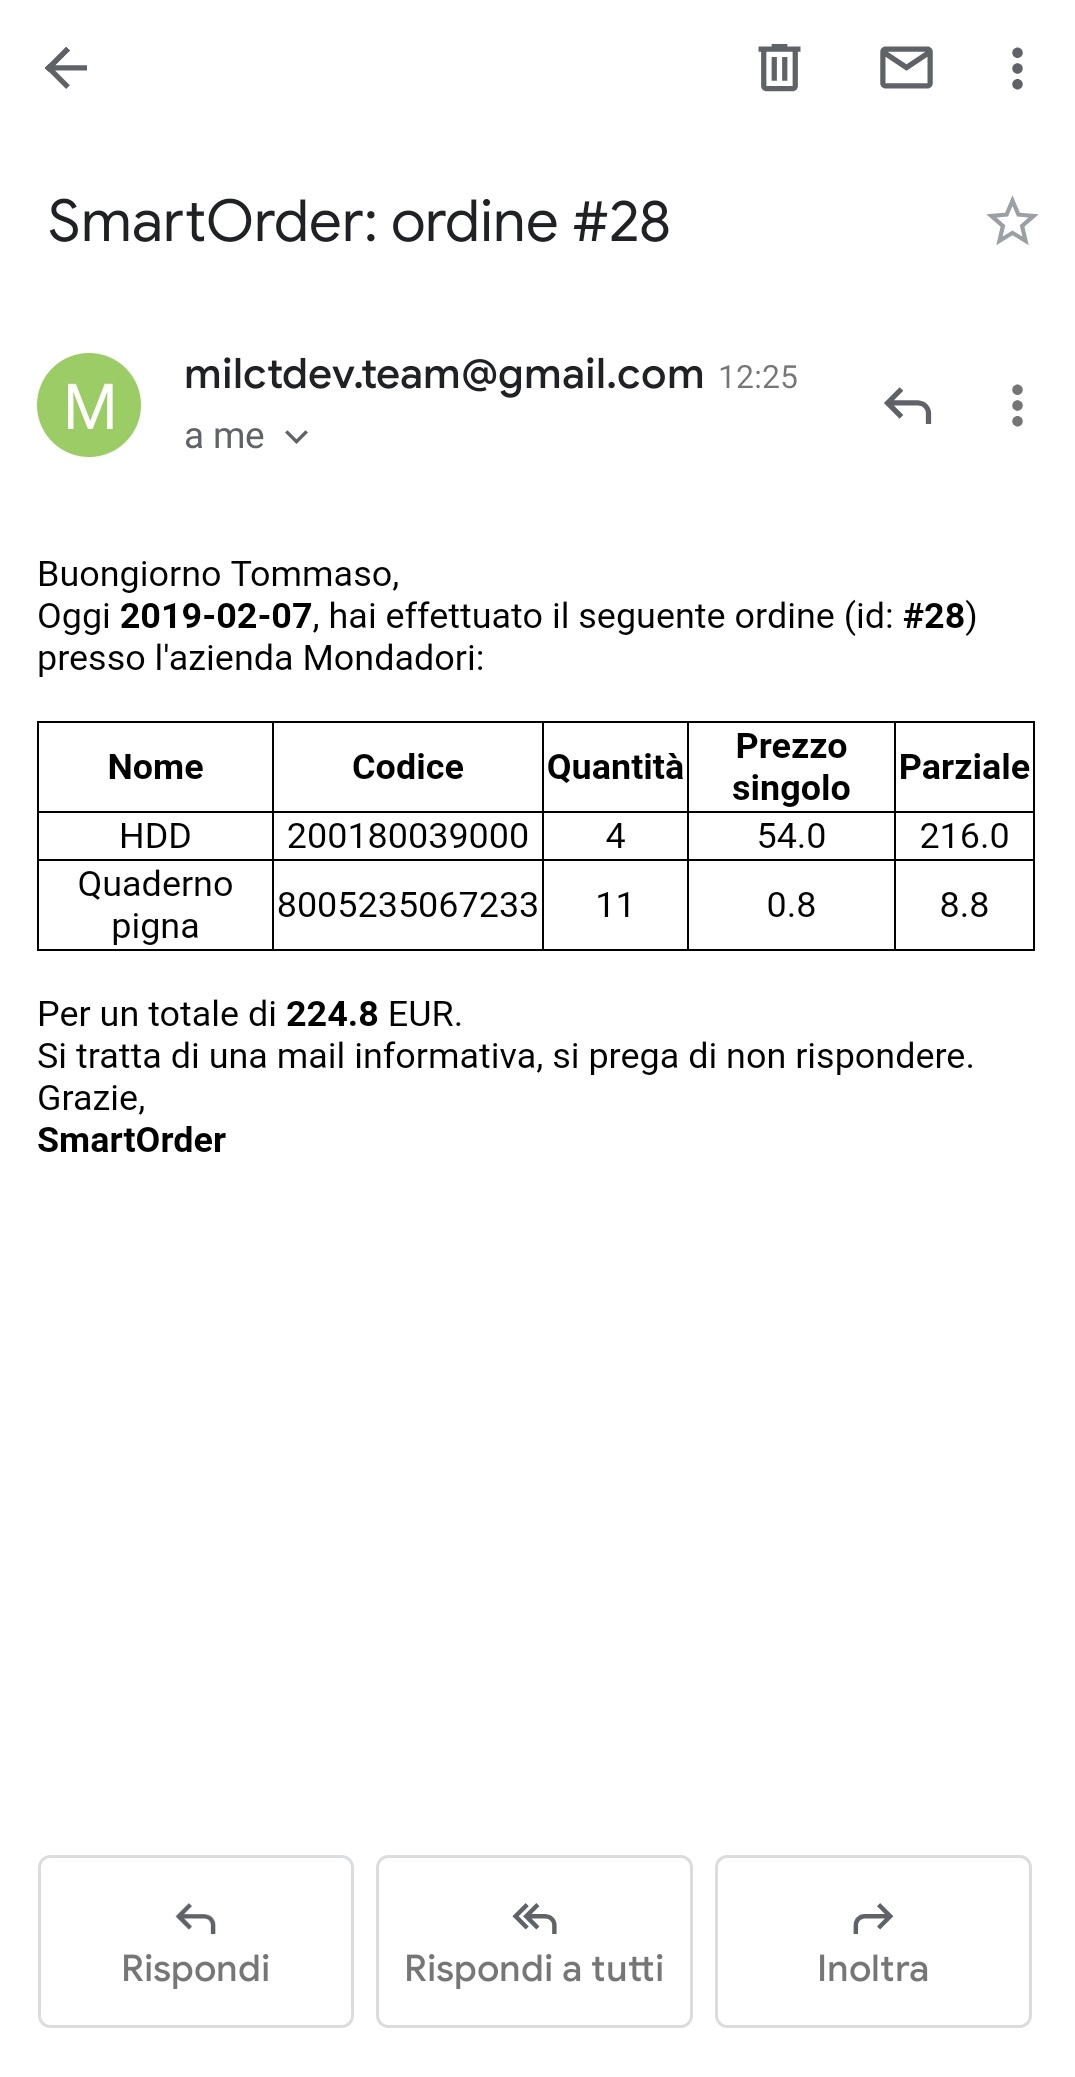
\includegraphics[width=0.4\columnwidth]{img/mail-utente}}
		\hspace*{2cm}
		\subfloat[\textit{Mail} ricevuta dall'azienda]{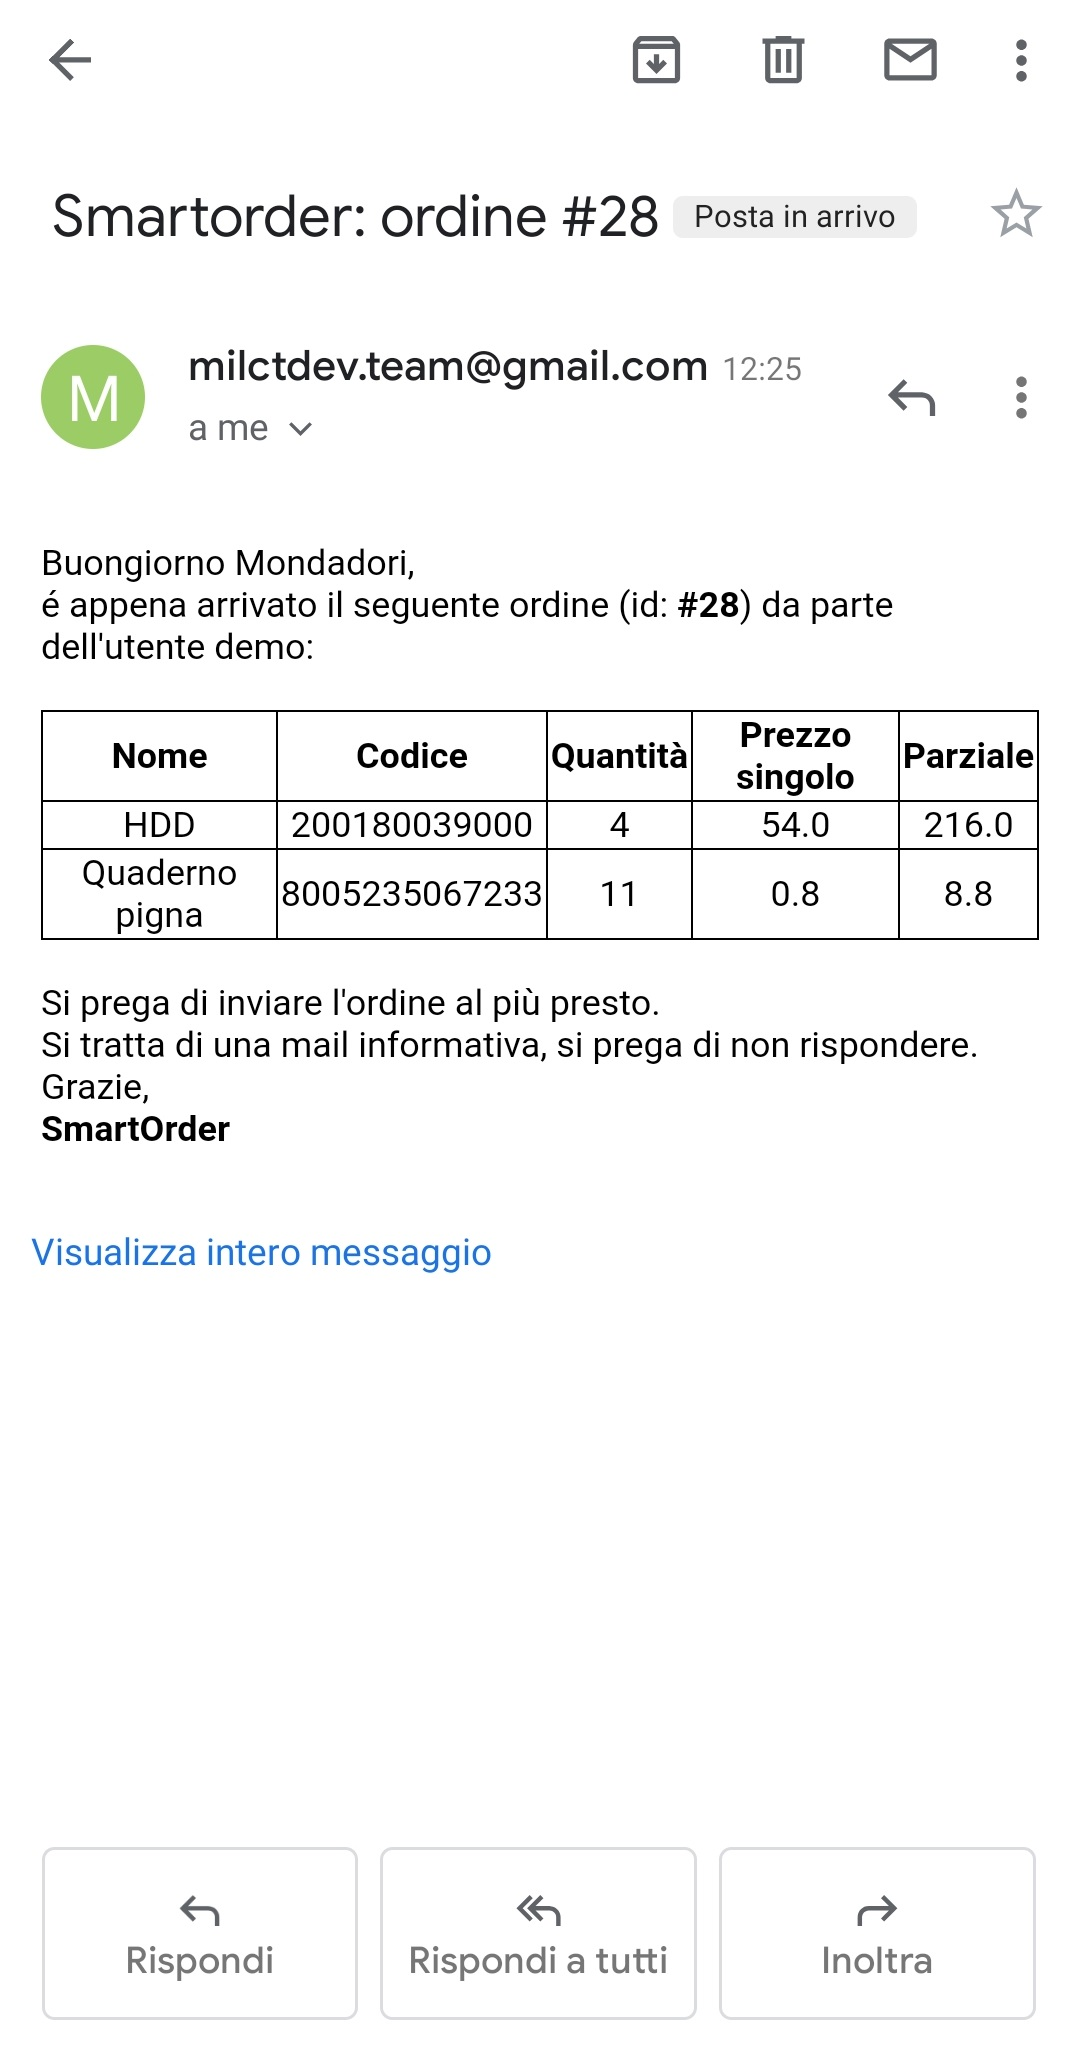
\includegraphics[width=0.4\columnwidth]{img/mail-azienda}}
		\caption{Tipologia di \textit{e-mail} inviate dall'applicazione}
		\label{fig:mail}
	\end{figure}
	
	\noindent Per testare lo scanner di codici a barre si consiglia di scansionare il seguente codice a barre. Tentando di scansionare altri codici si visualizzerà un messaggio d'errore, in quanto ogni nuovo \textit{barcode} deve essere registrato all'interno del \textit{database}.
	
	\begin{figure}[H] 
		\centering
		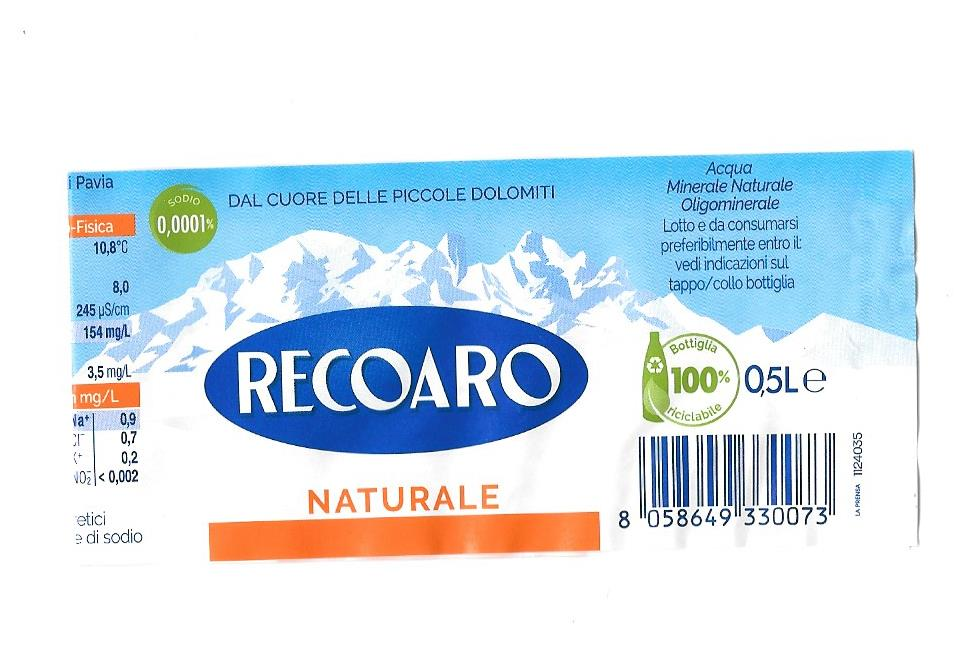
\includegraphics[width=0.8\columnwidth]{img/barcode}
		\caption{\textit{Barcode} per il test dello scanner}
		\label{fig:code}
	\end{figure}
	
	\noindent Infine si fa notare che il \textit{loader} dell'applicazione indica che \textit{SmartOrder} è in fase di scaricamento dati dal \textit{server} e sta momentaneamente attendendo una risposta per la costruzione della pagina. Il \textit{loader} è stato implementato proprio per fare in modo che l'utente non interagisca con l'applicazione prima della visualizzazione della pagina. Quindi, se si premesse qualche bottone prima dell'avvenuto caricamento, potrebbero accadere problemi di \textit{rendering}.
	
	\section{Progettazione frontend}
	
	Il \textit{frontend} è stato realizzato mediante utilizzo di tecnologie \textit{web}. \textit{HTML} e \textit{CSS} hanno predisposto l'interfaccia grafica, mentre \textit{JavaScript} ha permesso di implementare la logica applicativa.
	Le pagine realizzate sono le seguenti:
	\begin{itemize}
		\item \textit{index.html};
		\item \textit{login.html};
		\item \textit{homepage.html};
		\item \textit{order.html};
		\item \textit{article.html};
		\item \textit{articles.html};
		\item \textit{newpage.html};
		\item \textit{inventory.html}.
	\end{itemize}
	Ad ognuna di queste pagine è associato un foglio di stile e un \textit{file} \textit{Javascript}; inoltre sono presenti un \textit{file CSS} e un \textit{file Javascript} generali. Nelle prossime sezioni vengono descritte le funzionalità di \textit{SmartOrder}.
	
	\subsection{Login e tutorial}
	
	L'applicazione, una volta installata, è utilizzabile. All'avvio della stessa viene mostrata la pagina di \textit{login} per accedere al servizio. In questa schermata devono essere inserite le credenziali fornite dal proprio fornitore in fase di registrazione. La pagina presenta una \textit{checkbox} ``Resta collegato'' per evitare che ad ogni apertura dell'applicazione venga richiesto il \textit{login}. In seguito al \textit{login}, soltanto al primo avvio, viene mostrato un breve tutorial sul funzionamento dell'applicazione. In fondo al tutorial è presente un bottone che permette di iniziare ad utilizzare l'app. Nel caso in cui un utente si trovasse in difficoltà durante l'utilizzo dell'applicazione, è possibile trovare il tutorial nel menu della stessa. Completato il tutorial si viene reindirizzati al \textit{Carrello}.
	
	\subsection{Carrello}
	La pagina \textit{Carrello} è la pagina principale dell'applicazione e visualizza per ogni articolo in carrello la quantità decisa dall'utente, il prezzo e il prezzo parziale (prezzo unitario di un articolo x quantità dell'articolo stesso). Ogni articolo in carrello presenta due bottoni: 
	\begin{itemize}
		\item \textbf{MODIFICA}: permette di modificare l'articolo. Alla sua pressione si viene reindirizzati alla pagina per la modifica dell'articolo, dove è possibile modificarne la quantità. Una volta effettuata la modifica è necessario confermarla per apportarla definitivamente, premendo sul bottone ``Conferma'', oppure annullarla, tramite il bottone ``Annulla'';
		\item \textbf{ELIMINA}: permette di rimuovere l'articolo dal carrello. Se tale bottone viene premuto, verrà chiesta conferma prima di effettuare l'operazione. I motivi di questa scelta sono spiegati in sezione §\ref{butt}).
	\end{itemize}
	Inoltre, in questa pagina è presente un \textit{footer} contenente:
	\begin{itemize}
		\item il prezzo totale di tutti gli articoli inseriti nel carrello;
		\item un pannello di bottoni utilizzabili per la gestione del carrello:
		\begin{itemize}
			\item bottone \textit{Scan}: la spiegazione di questo pulsante è presente nella sezione successiva;
			\item bottone \textit{Svuota}: permette di svuotare il carrello. In seguito alla pressione viene chiesta conferma dell'azione;
			\item bottone \textit{Invia}: permette di inviare un ordine composto dagli articoli nel carrello. In seguito alla pressione viene chiesta conferma dell'azione. Dopo aver confermato si riceverà un'\textit{e-mail} contenente le informazioni relative all'ordine effettuato.
		\end{itemize}
	\end{itemize} 
	
	\subsubsection{Aggiunta di un articolo al carrello}
	È possibile aggiungere un articolo al carrello in due modi: 
	\begin{enumerate}
		\item tramite scansione del codice a barre in seguito alla pressione del bottone \textit{Scan} nella pagina \textit{Carrello}, accedibile dal menu dell'applicazione;
		\item dalla pagina \textit{Inventario}, accedibile tramite il menu dell'applicazione, selezionando l'articolo che si desidera aggiungere e inserendone la quantità nella pagina di aggiunta dell'articolo. Una volta immessa la quantità desiderata, è necessario premere su ``Conferma'' affinché l'articolo venga inserito nel carrello, oppure su ``Annulla'' per annullare l'inserimento del nuovo articolo. Nella pagina \textit{Inventario} è inoltre possibile ricercare un articolo, per nome o per codice, digitando la chiave di ricerca nella \textit{textbox} disposta in alto.
	\end{enumerate}
	La pagina per l'aggiunta di un articolo, che presenta la stessa interfaccia grafica della pagina per la modifica di un articolo, contiene le seguenti informazioni:
	\begin{itemize}
		\item nome dell'articolo: visualizzato in alto alla pagina;
		\item descrizione dell'articolo: visualizzata subito dopo il nome;
		\item pannello per l'inserimento della quantità: le modalità di interazione con questo pannello sono spiegate in sezione §\ref{tast};
		\item prezzo dell'articolo: visualizzato alla fine della pagina. Si tratta di un campo dinamico in quanto varia a seconda della quantità inserita.
	\end{itemize}
	\textbf{Attenzione}: nel caso in cui si cercasse di aggiungere al carrello un articolo già presente in esso, il sistema mostrerà un messaggio nel quale chiederà se si vuole modificare la quantità dello stesso.
	
	\subsection{Visualizzazione ordini}
	Dal menu dell'applicazione è possibile accedere alla lista di tutti gli ordini effettuati premendo sulla voce \textit{Ordini}. Alla sua pressione si verrà reindirizzati alla pagina \textit{Ordini}, dove per ogni ordine, vengono mostrate le seguenti informazioni:
	\begin{itemize}
		\item codice: è il codice che identifica univocamente l'ordine;
		\item data: è la data in cui è stato effettuato l'ordine;
		\item totale: è il totale in euro dell'ordine.
	\end{itemize} 
	La pagina permette di modificare la visualizzazione degli ordini, ordinandoli per data, dal più recente al meno recente, oppure per prezzo crescente. Per selezionare la tipologia di ordinamento è presente una \textit{select} in fondo alla pagina.
	Tramite il bottone ``DETTAGLI'', situato sulla destra di ogni ordine, è possibile consultare la lista degli articoli acquistati in quell'ordine. Alla sua pressione si verrà reindirizzati ad una pagina contenente le seguenti informazioni per ogni articolo acquistato:
	\begin{itemize}
		\item nome;
		\item quantità;
		\item prezzo;
		\item prezzo parziale.
	\end{itemize}

	\subsection{Inventario}
	
	Dal menu dell'applicazione è possibile accedere alla lista di tutti i prodotti venduti dalla propria azienda, premendo sulla voce \textit{Inventario}. Alla sua pressione si verrà reindirizzati alla pagina \textit{Inventario}, dove per ogni articolo, vengono mostrate le seguenti informazioni:
	\begin{itemize}
		\item codice: è il codice che identifica univocamente l'articolo;
		\item nome: è il nome dell'articolo;
		\item prezzo: è il prezzo unitario dell'articolo.
	\end{itemize}
	Infine, per ogni articolo, è possibile premere sul bottore ``APRI'', che permette di visualizzare informazioni dettagliate (descrizione) sullo stesso e di aggiungerlo al carrello. La pagina che viene aperta in seguito alla pressione del bottone è la pagina di aggiunta o modifica di un articolo, di cui si è già parlato. 
	
	\section{Mobile design}
	
	In questa sezione vengono descritte le scelte implementative effettuate ai fini di una corretta progettazione dell'interfaccia grafica. Questa sezione è suddivisa in varie sottosezioni e ognuna di esse descrive un elemento dell'interfaccia e le motivazioni alla base della sua progettazione.
	\medskip
	
	\noindent La maggior parte delle pagine dell'applicazione sono progettate nel seguente modo:
	\begin{itemize}
		\item la parte superiore presenta il pulsante menu sulla sinistra e il titolo della pagina al centro;
		\item la parte centrale presenta il contenuto informativo;
		\item la parte inferiore presenta un \textit{footer} che varia a seconda della pagina visualizzata.
	\end{itemize}
	
	\subsection{Bottoni} \label{butt}
	
	\begin{figure}[H] 
		\centering
		\subfloat[Bottoni presenti nel \textit{footer} della pagina \textit{Carrello} ]{
\includegraphics[width=0.4\columnwidth]{img/buttons-cart}}
		\hspace*{2cm}
		\subfloat[Bottoni presenti nel \textit{footer} delle pagine \textit{Aggiungi} e \textit{Modifica} articolo]{
\includegraphics[width=0.4\columnwidth]{img/buttons-add}}
		\caption{Bottoni nel \textit{footer}}
		\label{fig:buttons}
	\end{figure}
	Nelle pagine \textit{Carrello}, \textit{Modifica} e \textit{Aggiungi} sono presenti dei bottoni nella parte bassa dello schermo (Figura \ref{fig:buttons}). L'applicazione richiede una frequente modifica dei dati, quindi i controlli sono stati posizionati in una zona semplice da raggiungere e, seguendo la regola ``\textit{Content always on top}'', si è preferito inserire questi bottoni in basso, infrangendo così la convenzione che su \textit{Android} i controlli devono essere posizionati nella parte alta dello schermo. 
	\begin{figure}[H] 
		\centering
		\subfloat[Bottoni nella pagina \textit{Carrello} ]{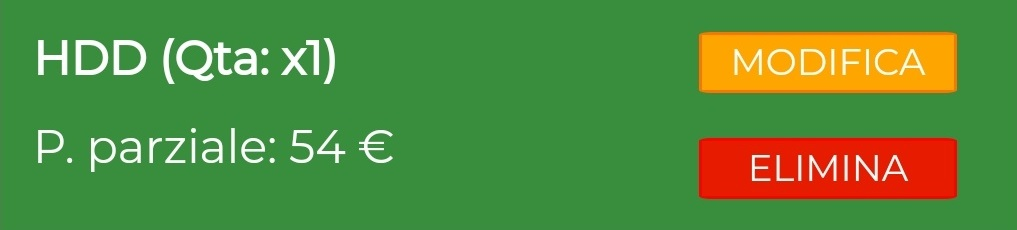
\includegraphics[width=0.3\columnwidth]{img/item-cart}}
		\hspace*{1cm}
		\subfloat[Bottoni nella pagina \textit{Ordini}]{
\includegraphics[width=0.3\columnwidth]{img/item-order}}
		\hspace*{1cm}
		\subfloat[Bottoni nella pagina \textit{Inventario}]{
\includegraphics[width=0.3\columnwidth]{img/item-inventory}}
		\caption{Bottoni nella parte centrale delle pagine}
		\label{fig:item-buttons}
	\end{figure}
	\noindent I bottoni presenti in Figura \ref{fig:item-buttons} sono situati nella parte centrale dello schermo. Essendo disposti nella \textit{comfort zone}, risultano facilmente raggiungibili e più piccoli rispetto ai bottoni del \textit{footer}, in quanto si è seguita l'immagine in Figura \ref{fig:dimvspos}. La dimensione è stata opportunamente scelta per fare in modo che l'utente non prema accidentalmente su di essi, in quanto possono cambiare lo stato del carrello oppure dare luogo all'apertura di nuove pagine. Nonostante la dimensione ridotta, sono comunque sufficientemente distanti da evitare \textit{tap} accidentali sui bottoni vicini. Infine, in caso si premesse sul bottone ``ELIMINA'' affianco ad un articolo nella pagina \textit{Carrello}, viene chiesta la conferma di eliminazione. Si tratta di un modo per rendere l'operazione reversibile.
	\begin{figure}[H] 
		\centering
		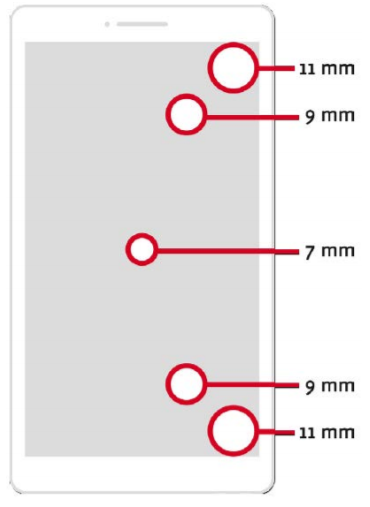
\includegraphics[width=0.3\textwidth]{img/dimvspos}
		\caption{Dimensione vs. posizione dei bottoni}
		\label{fig:dimvspos}
	\end{figure}

	\subsubsection{Bottone indietro}
	
	Poiché negli \textit{smartphone Apple} non è presente il tasto indietro, si è dovuto aggiungere lo stesso nella versione \textit{iOS} di \textit{SmartOrder}. La visualizzazione del bottone viene mostrata nell'immagine sottostante. Per lo stile del bottone e la sua posizione, il gruppo ha preso ispirazione dall'app \textit{mobile} Amazon per \textit{iOS}.
	
	\begin{figure}[H] 
		\centering
		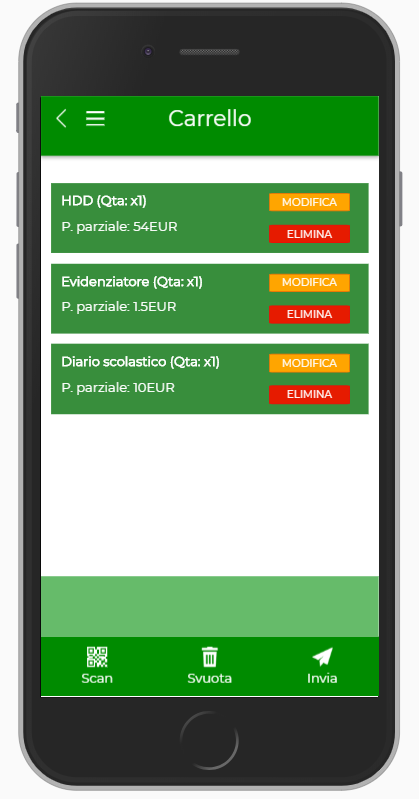
\includegraphics[width=0.4\textwidth]{img/apple-cart}
		\caption{Bottone indietro su \textit{iOS}}
		\label{fig:bottIndietro}
	\end{figure} 
	
	\subsection{Menu}
	
	\begin{figure}[H] 
		\centering
		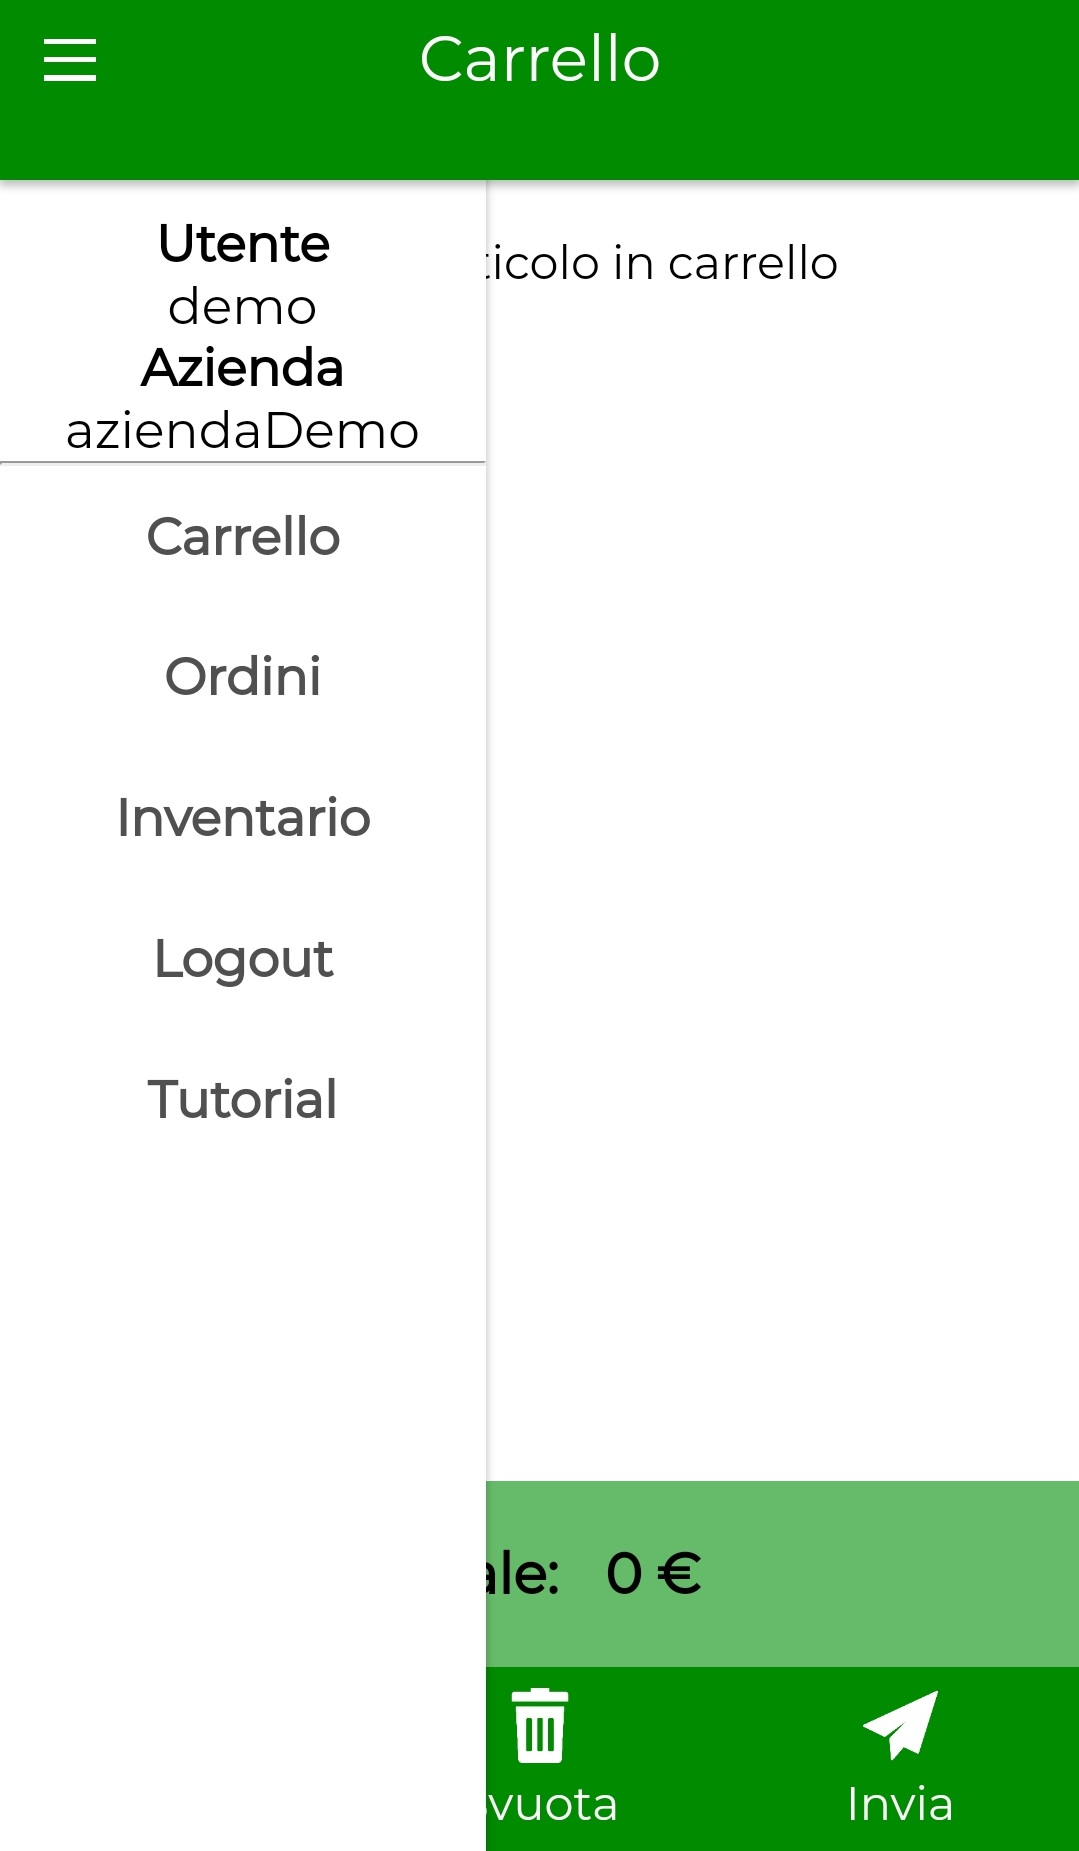
\includegraphics[width=0.3\textwidth]{img/menu}
		\caption{Menu dell'applicazione}
		\label{fig:menu}
	\end{figure}
	Il menu dell'applicazione è rappresentato in Figura \ref{fig:menu}. Per accederci è presente il classico bottone ``\textit{hamburger}'' in alto a sinistra di ogni pagina. Il menu è suddiviso in due parti: 
	\begin{itemize}
		\item informazioni relative all'utente che ha effettuato il \textit{login} nell'applicazione. In particolare, vengono visualizzati il nome dell'utente e il codice azienda del fornitore dello stesso. Queste informazioni non sono modificabili e pertanto sono state disposte nella parte alta del menu;
		\item insieme di \textit{link} che permettono di navigare tra le pagine dell'applicazione. In particolare, sono disponibili i \textit{link} al carrello, alla lista degli ordini e all'inventario. Inoltre, è possibile effettuare il \textit{logout} dall'applicazione o visionare nuovamente il tutorial. Questi bottoni sono stati posizionati nella parte centrale del menu (\textit{comfort zone}), in modo da essere facilmente accessibili quando il menu risulta aperto.
	\end{itemize}

	\subsection{Progressive disclosure}
	
	In generale, è buona prassi non affollare le interfacce. Al fine di perseguire questo obiettivo si è utilizzato il principio della \textit{progressive disclosure} (interfacce \textit{just-in-time}):
	\begin{itemize}
		\item nella pagina \textit{Ordini} è possibile visualizzare le informazioni essenziali per poter identificare un ordine. Per accedere ai dettagli risulta necessario un ulteriore \textit{tap};
		\item nella pagina \textit{Inventario} è possibile visualizzare le informazioni essenziali per poter identificare un articolo. Per accedere ai dettagli dello stesso, o per aggiungerlo al carrello, risulta necessario un ulteriore \textit{tap}.
	\end{itemize}
	
	\subsection{Uso della tastiera} \label{tast}
	
	L'utilizzo della tastiera è stato limitato a tre casi:
	\begin{itemize}
		\item inserimento delle credenziali in fase di \textit{login};
		\item ricerca di un articolo;
		\item inserimento o modifica della quantità nelle pagine \textit{Aggiungi} e \textit{Modifica}, rispettivamente. In questo caso la tastiera permette un veloce inserimento di grandi quantità.
	\end{itemize}
	Per l'inserimento della quantità è stata predisposta una seconda modalità. Sono stati messi a disposizione due pulsanti (+/-), i quali permettono di aumentare o diminuire la quantità, rispettivamente. Tramite questa modalità è possibile inserire velocemente piccole quantità.
	
	\subsection{Aiuti per l'utente}
	
	Al primo accesso di un utente all'applicazione, viene visualizzato il tutorial della stessa. Esso fornisce istruzioni rilevanti per l'utilizzo dell'applicazione e risulta breve, in quanto l'applicazione è stata progettata per essere massimamente intuitiva. Alla fine del tutorial è presente un bottone che permette di iniziare ad utilizzare l'applicazione. Il tutorial sarà comunque disponibile dal menu, nel caso in cui l'utente non ricordasse come utilizzare l'app.
	
	\subsection{Elementi nativi}
	
	Gli elementi nativi dell'applicazione sono la fotocamera, per la scansione del codice a barre, e i \textit{dialog}, per la visualizzazione di messaggi informativi o di conferma. Inoltre, si è dovuta monitorare la rete del dispositivo. Per rendere questi elementi nativi si sono utilizzati i seguenti \textit{plugin} di \textit{PhoneGap}:
	\begin{itemize}
		\item \textit{dialogs}: fornisce un'interfaccia per convertire gli \textit{alert} e i \textit{confirm} delle pagine web in \textit{dialog box} nativi. In questo modo è stato possibile customizzare i titoli e le etichette dei pulsanti nei \textit{dialog};
		\item \textit{barcodescanner}: fornisce un'interfaccia per accedere nativamente alla fotocamera del dispositivo ed effettuare la scansione di un codice a barre;
		\item \textit{network information}: fornisce un'interfaccia per accedere alle informazioni relative alle connessioni \textit{Wi-Fi} e cellulare del dispositivo.
	\end{itemize}

	\subsection{Gesture}
	
	Per l'applicazione è stata implementata una sola tipologia di \textit{gesture}, ossia lo \textit{scroll} per scorrere all'interno delle varie pagine. Questa \textit{gesture} è presente nella pagine \textit{Carrello}, \textit{Ordini}, \textit{Inventario} e per la descrizione nella pagina di aggiunta o modifica di un articolo in carrello.
	Il gruppo non è riuscito ad implementare la \textit{gesture} \textit{swipe right} per l'apertura del menu. Quest'ultima risulta difficilmente realizzabile tramite il solo utilizzo di \textit{JavaScript} puro.
	
	\subsection{Considerazioni finali}
	
	Si ritiene che l'applicazione soddisfi i primi tre livelli della piramide di \textit{Maslow} rimappata sui bisogni degli utenti, ovvero che sia funzionale, affidabile e usabile.
	
	\section{Backend}
	
	Per l'implementazione del \textit{backend} si è deciso di appoggiarsi ad \textit{Amazon Web Services (AWS)}, in quanto tramite l'\textit{account} universitario è possibile usufruire dei servizi offerti gratuitamente.
	
	\subsection{Architettura}
	
	Il \textit{backend} della piattaforma presenta la seguente architettura:
	\begin{itemize}
		\item un \textit{server cloud AWS EC2} configurato con \textit{Windows Server 2017};
		\item un'istanza \textit{AWS RDS} contenente un \textit{database Microsoft SQL Server}.
	\end{itemize}
	All'interno dell'istanza \textit{AWS EC2} sono stati installati:
	\begin{itemize}
		\item un \textit{server web Apache Tomcat}: esso permette di eseguire un \textit{web service} scritto in linguaggio \textit{Java}, il quale si occupa di captare le richieste \textit{HTTP} che provengono dall'applicazione, di elaborarle e di rispondere ad esse tramite stringhe \textit{JSON} costruite sulla base di \textit{query} effettuate su \textit{database};
		\item il linguaggio \textit{Java}: necessario per il funzionamento di \textit{Apache Tomcat} e per l'esecuzione del \textit{web service}.
	\end{itemize}

	\subsection{Web service}
	
	Per lo sviluppo del \textit{web service} si sono utilizzati gli oggetti \textit{servlet Java}. Essi permettono di captare richieste \textit{HTTP} e di rispondere ad esse tramite stringhe in formato \textit{JSON}. Il servizio web è costituito dai seguenti \textit{package}:
	\begin{itemize}
		\item \textit{dbConnection}: \textit{package} contenente una classe utilizzabile per connettersi ed interagire con un \textit{database SQL Server};
		\item \textit{servlet}: \textit{package} contenente le classi \textit{servlet} del servizio web;
		\item \textit{utility}: \textit{package} contenente le classi utilità del servizio web.
	\end{itemize}

	\subsubsection{Servlet}
	
	In questa sezione vengono descritte le classi \textit{servlet} e per ognuna di esse vengono indicate le seguenti caratteristiche:
	\begin{itemize}
		\item \textbf{End-point}: \textit{end-point} che identifica il \textit{servlet}. L'\textit{end-point} è utilizzabile per comunicare con lo specifico \textit{servlet} all'interno del \textit{web service};
		\item \textbf{Parametri}: lista dei parametri che devono essere inseriti nella richiesta \textit{HTTP} al fine di comunicare correttamente con il \textit{servlet};
		\item \textbf{Funzionalità}: una breve descrizione delle operazioni eseguite dal \textit{servlet} e della tipologia di risposta che restituisce.
	\end{itemize}

	\begin{enumerate}
		\item \textbf{AggiuntaModificaArticolo.java}
		\begin{itemize}
			\item \textbf{End-point}: \textit{/AggiuntaModificaArticolo}
			\item \textbf{Parametri}:
			\begin{itemize}
				\item codice azienda: è il codice che identifica univocamente il \textit{database} del fornitore corrispondente all'utente loggato;
				\item \textit{query}: è la \textit{query} di inserimento o modifica di un articolo nel carrello dell'utente loggato.
			\end{itemize}
			\item \textbf{Funzionalità}: il \textit{servlet} si connette al database identificato dal codice azienda fornito ed effettua la \textit{query} fornita su di esso. Se la \textit{query} va a buon fine restituisce una stringa \textit{JSON} contenente codice 1 (operazione andata a buon fine), altrimenti codice 0 (operazione fallita).
		\end{itemize}
	
		\item \textbf{Autenticazione.java}
		\begin{itemize}
			\item \textbf{End-point}: \textit{/Autenticazione}
			\item \textbf{Parametri}:
			\begin{itemize}
				\item \textit{username}: è la \textit{username} che l'utente ha inserito in fase di \textit{login};
				\item \textit{password}: è la \textit{password} che l'utente ha inserito in fase di \textit{login}.
			\end{itemize}
			\item \textbf{Funzionalità}: il \textit{servlet} si connette al \textit{database} ideato per la gestione dell'autenticazione e cerca all'interno di esso le credenziali fornite. Se le credenziali vengono identificate viene restituita una stringa \textit{JSON} contenente codice 0, altrimenti ci possono essere le seguenti possibilità:
			\begin{itemize}
				\item codice 1: la \textit{password} inserita dall'utente non è quella corretta;
				\item codice 2: la \textit{username} inserita dall'utente è inesistente.
			\end{itemize}
		\end{itemize}
	
		\item \textbf{EliminazioneArticoli.java}
		\begin{itemize}
			\item \textbf{End-point}: \textit{/EliminazioneArticoli}
			\item \textbf{Parametri}:
			\begin{itemize}
				\item \textit{username}: è la \textit{username} dell'utente loggato;
				\item codice azienda: è il codice che identifica univocamente il \textit{database} del fornitore corrispondente all'utente loggato;
				\item lista codici: è la lista dei codici a barre dei prodotti che devono essere rimossi dal carrello dell'utente loggato.
			\end{itemize}
			\item \textbf{Funzionalità}: il \textit{servlet} si connette al \textit{database} identificato dal codice azienda fornito ed elimina dalla tabella \textit{contenutoCarrelli} gli articoli corrispondenti ai codici e alla \textit{username} forniti. Infine restituisce una stringa \textit{JSON} contenente codice 1 se l'eliminazione è andata a buon fine, altrimenti codice 0.
		\end{itemize}
	
		\item \textbf{InvioOrdine.java}
		\begin{itemize}
			\item \textbf{End-point}: \textit{/InvioOrdine}
			\item \textbf{Parametri}:
			\begin{itemize}
				\item \textit{username}: è la \textit{username} dell'utente loggato;
				\item codice azienda: è il codice che identifica univocamente il \textit{database} del fornitore corrispondente all'utente loggato;
				\item totale: è il totale dell'ordine che l'utente ha deciso di inviare.
			\end{itemize}
			\item \textbf{Funzionalità}: il \textit{servlet} si connette al \textit{database} identificato dal codice azienda fornito e crea in \textit{database} un nuovo ordine contenente gli articoli presenti nel carrello dell'utente identificato dalla \textit{username} fornita. Infine invia un'\textit{e-mail} di notifica dell'ordine sia all'utente identificato dalla \textit{username} fornita che all'azienda identificata dal codice azienda fornito.
		\end{itemize}
	
		\item \textbf{PrelevaArticoliAzienda.java}
		\begin{itemize}
			\item \textbf{End-point}: \textit{/PrelevaArticoliAzienda}
			\item \textbf{Parametri}:
			\begin{itemize}
				\item codice azienda: è il codice che identifica univocamente il \textit{database} del fornitore corrispondente all'utente loggato;
			\end{itemize}
			\item \textbf{Funzionalità}: il \textit{servlet} si connette al \textit{database} identificato dal codice azienda fornito e restituisce una stringa \textit{JSON} contenente le informazioni sugli articoli venduti dall'azienda.
		\end{itemize}
	
		\item \textbf{PrelevaDatiOrdine.java}
		\begin{itemize}
			\item \textbf{End-point}: \textit{/PrelevaDatiOrdine}
			\item \textbf{Parametri}:
			\begin{itemize}
				\item codice azienda: è il codice che identifica univocamente il \textit{database} del fornitore corrispondente all'utente loggato;
				\item codice ordine: è il codice dell'ordine di cui si vogliono conoscere i dettagli.
			\end{itemize}
			\item \textbf{Funzionalità}: il \textit{servlet} si connette al database identificato dal codice azienda fornito e restituisce una stringa \textit{JSON} contenente le informazioni relative all'ordine corrispondente al codice ordine fornito.
		\end{itemize}
	
		\item \textbf{PrelevaOrdini.java}
		\begin{itemize}
			\item \textbf{End-point}: \textit{/PrelevaOrdini}
			\item \textbf{Parametri}:
			\begin{itemize}
				\item \textit{username}: è la \textit{username} dell'utente loggato;
				\item codice azienda: è il codice che identifica univocamente il \textit{database} del fornitore corrispondente all'utente loggato;
			\end{itemize}
			\item \textbf{Funzionalità}: il \textit{servlet} si connette al \textit{database} identificato dal codice azienda fornito e restituisce una stringa \textit{JSON} contenente le informazioni relative agli ordini effettuati dall'utente corrispondente alla \textit{username} fornita.
		\end{itemize}
	
		\item \textbf{PrelievoInfoArticoli.java}
		\begin{itemize}
			\item \textbf{End-point}: \textit{/PrelievoInfoArticoli}
			\item \textbf{Parametri}:
			\begin{itemize}
				\item \textit{username}: è la \textit{username} dell'utente loggato;
				\item codice azienda: è il codice che identifica univocamente il \textit{database} del fornitore corrispondente all'utente loggato;
			\end{itemize}
			\item \textbf{Funzionalità}: il \textit{servlet} si connette al \textit{database} identificato dal codice azienda fornito e restituisce una stringa \textit{JSON} contenente le informazioni relative agli articoli nel carrello dell'utente identificato dalla \textit{username} fornita.
		\end{itemize}
	
		\item \textbf{PrelievoInfoArticolo.java}
		\begin{itemize}
			\item \textbf{End-point}: \textit{/PrelievoInfoArticolo}
			\item \textbf{Parametri}:
			\begin{itemize}
				\item codice articolo: è il codice dell'articolo di cui si vogliono conoscere i dettagli;
				\item codice azienda: è il codice che identifica univocamente il \textit{database} del fornitore corrispondente all'utente loggato;
			\end{itemize}
			\item \textbf{Funzionalità}: il \textit{servlet} si connette al \textit{database} identificato dal codice azienda fornito e restituisce una stringa \textit{JSON} contenente le informazioni relative all'articolo corrispondente al codice articolo fornito.
		\end{itemize}
	\end{enumerate}
	
	\subsubsection{Utility}
	Il \textit{package} \textit{utility} contiene le seguenti classi utilità:
	\begin{itemize}
		\item \textit{\textbf{GetDb}}: classe contenente un metodo statico che restituisce la stringa di connessione dal \textit{database} di autenticazione;
		\item \textit{\textbf{SendMail}}: classe che fornisce un'interfaccia per l'invio di \textit{e-mail} tramite un \textit{server SMTP} di \textit{AWS}.
	\end{itemize}
	
	\subsection{Database}
	
	Per la gestione di ordini, utenti e articoli venduti dai vari fornitori sono stati utilizzati dei \textit{database Microsoft SQL Server}. In questa sezione vengono descritti i seguenti \textit{database}:
	\begin{itemize}
		\item \textit{database} di autenticazione;
		\item \textit{database} aziendale.
	\end{itemize}
	
	\subsubsection{Database per l'autenticazione}
	
	Il \textit{database} per l'autenticazione contiene le credenziali e le anagrafiche degli utenti registrati e le informazioni dei fornitori registrati all'applicazione. Questo \textit{database} contiene le seguenti tabelle:
	\begin{itemize}
		\item aziende: contiene le informazioni delle aziende registrate a \textit{SmartOrder}. La tabella contiene i seguenti attributi:
		\begin{itemize}
			\item codAzienda (chiave primaria): è un codice che identifica univocamente l'azienda. Esso viene fornito all'azienda in fase di registrazione all'applicazione;
			\item nome: è il nome dell'azienda;
			\item via: è la via dove è situata la sede principale dell'azienda;
			\item civico: è il civico dove è situtata la sede principale dell'azienda;
			\item comune: è il comune dove è situata la sede principale dell'azienda;
			\item provincia: è la provincia dove è situata la sede principale dell'azienda;
			\item CAP: è il codice postale dove è situata la sede principale dell'azienda;
			\item \textit{mail}: è la \textit{mail} che l'azienda ha fornito in fase di registrazione;
			\item telefono: è il numero di telefono che l'azienda ha fornito in fase di registrazione.
		\end{itemize}
		\item \textit{users}: contiene le informazioni relative agli utenti registrati a \textit{SmartOrder}. La tabella contiene i seguenti attributi:
		\begin{itemize}
			\item \textit{username} (chiave primaria): è il nome utente che è stato fornito all'utente in fase di registrazione;
			\item \textit{password}: è la \textit{password} che è stata fornita all'utente in fase di registrazione;
			\item \textit{mail}: è la \textit{mail} che l'utente ha fornito in fase di registrazione;
			\item codAzienda: è il codice dell'azienda presso cui l'utente è cliente;
			\item cellulare: è il numero di cellulare che l'utente ha fornito in fase di registrazione;
			\item nome: è il nome dell'utente;
			\item cognome: è il cognome dell'utente;
			\item via: è la via di residenza dell'utente;
			\item civico: è il civico di residenza dell'utente;
			\item comune: è il comune di residenza dell'utente;
			\item provincia: è la provincia di residenza dell'utente;
			\item CAP: è il codice postale di residenza dell'utente.
		\end{itemize}
	\end{itemize}
	
	\subsubsection{Database aziendale}
	
	Il \textit{database} aziendale contiene le informazioni relative agli articoli venduti e agli ordini effettuati presso uno specifico fornitore. Per cui, nel \textit{server} è presente un \textit{database} di questa tipologia per ogni fornitore registrato all'applicazione. Questo \textit{database} contiene le seguenti tabelle:
	\begin{itemize}
		\item articoli: contiene le informazioni relative agli articoli venduti dall'azienda. La tabella contiene i seguenti attributi:
		\begin{itemize}
			\item nome: è il nome dell'articolo;
			\item \textit{barCode} (chiave primaria): è il codice a barre dell'articolo;
			\item prezzo: è il prezzo dell'articolo;
			\item descrizione: è la descrizione dell'articolo.
		\end{itemize}
		\item contenutoCarrelli: contiene le informazioni relative al contenuto dei carrelli degli utenti dell'azienda. La tabella contiene i seguenti attributi:
		\begin{itemize}
			\item idRiga (chiave primaria): è un identificativo autoincrementante che funge unicamente da chiave primaria;
			\item \textit{barCode}: è il codice a barre dell'articolo in carrello;
			\item quantità: è la quantità scelta dall'utente per l'articolo in carrello;
			\item \textit{username}: è la \textit{username} dell'utente che ha inserito in carrello l'articolo.
		\end{itemize}
		\item contenutoOrdini: contiene le informazioni relative al contenuto degli ordini effettuati presso l'azienda. La tabella contiene i seguenti campi:
		\begin{itemize}
			\item idRiga (chiave primaria): è un identificativo autoincrementante che funge unicamente da chiave primaria;
			\item codiceOrdine: è il codice dell'ordine in cui é presente l'articolo;
			\item \textit{barCode}: è il codice a barre dell'articolo all'interno dell'ordine;
			\item quantità: è la quantità ordinata per l'articolo.
		\end{itemize}
		\item ordini: contiene le informazioni relative agli ordini effettuati presso l'azienda. La tabella contiene i seguenti campi:
		\begin{itemize}
			\item codiceOrdine (chiave primaria): è il codice che identifica univocamente l'ordine presso l'azienda;
			\item data: è la data in cui l'ordine è stato effettuato;
			\item \textit{username}: è la \textit{username} dell'utente che ha effettuato l'ordine;
			\item totale: è il totale in euro dell'ordine.
		\end{itemize}
	\end{itemize}
	
	\section{Conclusioni}
	
	Vi è la consapevolezza che l'interfaccia grafica possa essere resa più accattivante. L'implementazione della stessa poteva risultare più semplice tramite l'utilizzo di un altro \textit{framework}, come ad esempio \textit{React Native}. Il \textit{framework} scelto ha comunque permesso di realizzare un'interfaccia usabile in tempi ristretti. Il gruppo ritiene di aver realizzato una buona applicazione, che potrebbe risultare utile ad aziende ed utenti nel contesto per cui è stata progettata e implementata. Tra gli sviluppi futuri vi sono:
	\begin{enumerate}
		\item utilizzo di icone personalizzate;
		\item utilizzo di una \textit{palette} di colori definita a priori;
		\item implementazione di \textit{gesture swipe right} e \textit{swipe left} per l'eliminazione di articoli dal carrello;
		\item implementazione della \textit{gesture long press} per la modifica di un articolo in carrello;
		\item implementazione della \textit{gesture swipe right} per l'apertura del menu.
	\end{enumerate} 
\end{document}